\section{Results}

Implementation of the our approach is provided in the \texttt{R} package
\href{https://dajmcdon.github.io/rtestim/}{\texttt{rtestim}}. All experiments
are run in \texttt{R} with version 4.3.1 on Cedar cluster provided by Compute
Canada \attn{requires attribution in the acknowledgements, possibly a citation}.
The \texttt{R} packages used for simulation and real-data application are
versions \texttt{EpiEstim\_2.2-4}, \texttt{EpiLPS\_1.2.0}, and
\texttt{rtestim\_0.0.3}. 


\subsection{Simulation settings}

% problem settings
%% Rt
We simulate four scenarios of the time-varying effective reproduction numbers,
intended to mimic different epidemics. The first two scenarios are simple cases
that are rapidly controlled by intervention, where the graphical curves consist
of one discontinuity and two segments. Scenario 1 has constant $\calR_t$ before
and after an intervention, while Scenario 2 grows exponentially, then decays.
The other two scenarios are more complicated, where more waves in the epidemics
are involved. Scenario 3 has four linear segments with three discontinuities,
which reflect the effect of an intervention, resurgence to rapid transmission,
and finally suppression of pandemic. Scenario 4 involves sinusoidal waves
throughout the epidemic.
% motivation
The first three scenarios and the last scenario are motivated by
\citep{parag2021improved, gressani2022epilps} respectively. 
% name the scenarios
We name the four scenarios as (1) 2-segment constant, (2) 2-segment exponential curve, (3) 4-segment linear, and (4) periodic respectively. 

In all cases, the times of observation are regular, and consider epidemics of
length $n=300$. Specifically, in Scenario 1, $\calR_t = 2, 0.8$ before and after
$t=70$. In Scenario 2, $\calR_t$ increases and decreases exponentially with
rates $0.015, 0.005$ pre and post $t=50$. In Scenario 3, $\calR_t$ reduces from
$2.5$ to $2$ linearly between $t\in[1,60]$, falls to $0.8$ at $t=61$ and goes
linearly down to $0.6$ until $t=110$, resurges to $1.7$ at $t=111$ and grows
linearly back to $2$ until $t=150$, and then drops to $0.9$ at $t=151$ and
descends to $0.5$ until the end. In Scenario 4, $\calR_t$ is realization of the
continuous, periodic curve generated by the function $$\calR(t) = 0.2 \lr{
\lr{\sin(\frac{\pi t}{12}) + 1} + \lr{2 \sin\lr{\frac{\pi t}{6}} + 2} + \lr{3
\sin(\frac{\pi t}{1.2}) + 3} }$$ at equally spaced points $t\in [0,10]$. These
settings are illustrated in the left column of \autoref{fig:samples}.


%% other problem settings
We assume that the serial interval follows Gamma distribution with fixed shapes
and scales $(3,3)$, $(2.5,2.5)$, $(3.5,3.5)$ and $(3.5,3.5)$ for Scenarios 1--4
respectively. We consider all epidemics starting from $y_1=2$ cases and
generating until timepoints $t=300$. We compute the expected incidence
$\Lambda_t$ using the renewal equation, and generate the incidence samples from
the Poisson distribution $y_t\sim \textrm{Pois}(\Lambda_t)$. To verify the
performance of our model under the violation of this distributional assumption
of incidence, we also generate incidence samples using the negative Binomial
distribution with dispersion size 5, i.e., $y_t\sim \textrm{NB}(\Lambda_t,
\textrm{size}=5)$. We generate 50 random samples for each setting of
experiments, resulting in 400 total experiments. An example of each effective
reproduction number scenario with a single corresponding Poisson and negative
Binomial sample incidence sequence are displayed in \autoref{fig:samples}. 

\begin{figure}[hp!]
    \centering
    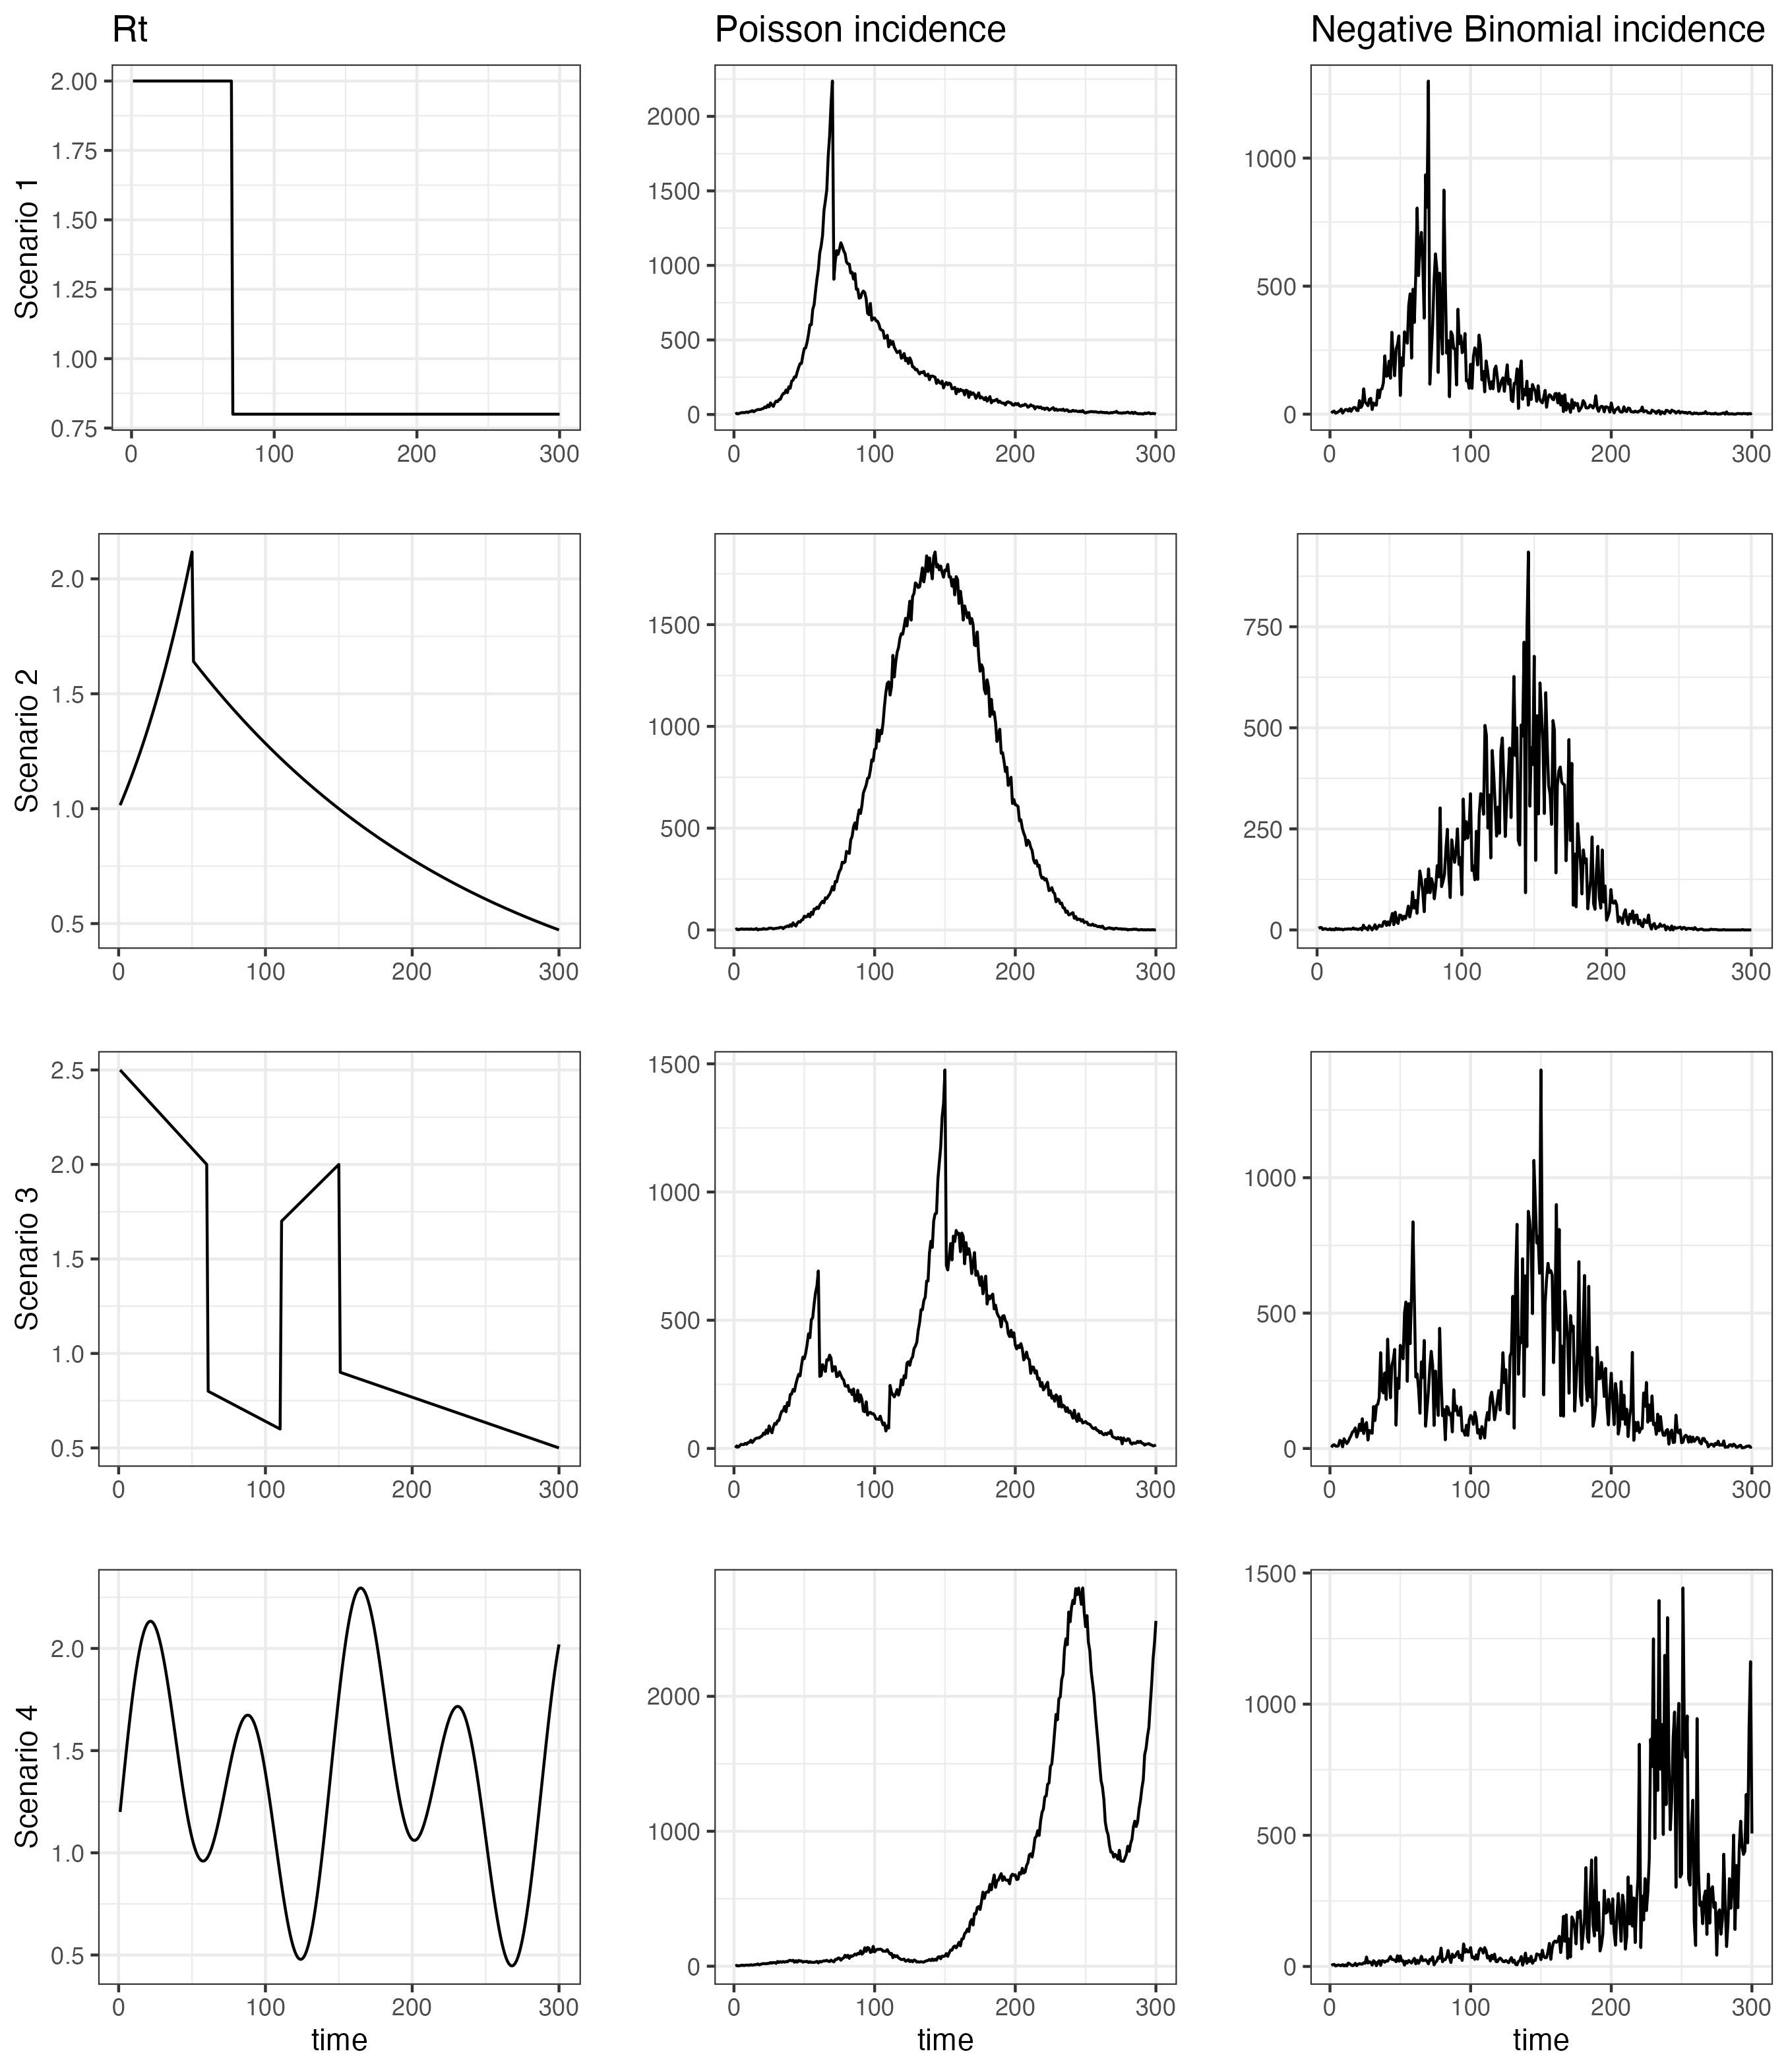
\includegraphics[width=.9\textwidth]{fig/plot_samples.png}
    \caption{The effective reproduction numbers (left column) and corresponding
    sample incident cases drawn from a  Poisson (middle column) or negative
    Binomial (right column) distribution. The rows correspond to the four
    $\calR_t$ settings.} 
    \label{fig:samples}
\end{figure}

% algorithm settings
%% competitors and their settings
We compare \RtEstim\ to \EpiEstim\ and \EpiLPS. Unfortunately,
\texttt{EpiFilter} frequently fails to converge due to the large case counts in
many simulations. \EpiEstim\ estimates the posterior distribution of effective
reproduction numbers given a Gamma prior and Poisson distributed incidences. It
estimates the reproduction number over a sliding window, assuming the
reproduction number is constant during the specific time window. A longer
sliding window averages out more fluctuations, leading to smoother estimates,
whereas, a shorter sliding window is more responsive to sudden spikes or
declines. We tried the default, a weekly sliding window, as well as a monthly
window. However, since neither considerably outperform the other across all
scenarios, we defer the monthly case to the Appendix. \EpiLPS\ is another
Bayesian approach that estimates P-splines coupled with Laplace approximations
of the conditional posterior based on the negative Binomial likelihood. For
\RtEstim\ on the four scenarios respectively, we estimate (1) piecewise constant
$k=0$, (2) piecewise linear \& cubic $k=1,3$, (3) piecewise linear $k=1$ and (4)
piecewise cubic polynomials $k=3$. In each case, we examine a grid of 50
$\lambda$s, selecting the best using cross validation. For all models and
problems, we use the generation interval distribution used to create the data. 

% KL for exponential family: 
To measure estimation accuracy, we compare $\widehat{\calR}$ to $\calR$ using
the Kullback-Leibler (KL) divergence: a standard metric that measures the
distance between two probability distributions. Since $\calR_t$ can be regarded
as the expectation of Poisson distribution, we use the mean KL divergence for
Poisson distributions (averaged across all coordinates) to measure the accuracy
of the $\calR_t$ estimates: $$\frac{1}{n} D_{KL}(\widehat{\calR} \Vert \calR) =
\frac{1}{n}\sum_{t=1}^n \widehat{\calR}_t \log\left(\frac{\widehat{\calR}_t}
{\calR_t}\right) + {\calR}_t - \widehat{\calR}_t,$$ \attn{I think the above
formula is close but wrong. Check, but I think you need to multiply everything
inside the sum by $\eta_t$, and you should reverse the order (expectation under
the truth). This suggests using (letting $w_t = \eta_t / \sum_t \eta_t$):
$$ D_{KL}(\calR \Vert \widehat{\calR}) = \sum_{t=1}^n w_t \left( \calR_t
\log\left(\frac{\calR_t}{\widehat{\calR}_t}\right) + \widehat{\calR}_t -
\calR_t\right)$$} where $\calR := \left\{ \calR_t \right\}_{t=1}^n$.
%It coincides with the Bregman distance $D_{KL}(\theta_0 || \theta_1) = \varphi(\theta_1) - \varphi(\theta_0) - (\theta_1 - \theta_0)^{\top} \varphi'(\theta_0)$, where $\theta_0,\theta_1$ are natural parameters of the same kind of exponential-family distributions \citep{sadhanala2022exponential}. 
To fairly compare across methods, we drop the estimates during the first
week because estimates from \EpiEstim\ do not begin until $t=8$ (using a weekly
window). KL-divergence is more appropriate for measuring accuracy because it
connects directly to the Poisson likelihood used to generate the data, whereas
standard measures like the mean-squared error correspond to Gaussian data. This
has the effect of increasing the relative cost of mistakes when $\Lambda_t$ is small.
%For negative Binomial cases, we use KL divergence to measure the distances between negative Binomial distributions given the %dispersion rate $\phi$, i.e., 
%\begin{align*}
%    \frac{1}{n} D^{\ast}_{KL}\lr{\hat{\calR}|| \calR} = \frac{1}{n}\sum_{t=1}^n \hat{\calR}_t \log \left(\frac{\hat{\calR}_t}%{\calR_t}\right) + \lr{\hat{\calR}_t + \phi} \log\lr{\frac{\hat{\calR}_t + \phi}{\calR_t + \phi}}. 
%\end{align*}
Other details of the experimental settings are deferred to the Appendix. 

%\subsubsection*{Cross Validation}
\attn{I think this goes to the Appendix too.}
We run leave-third-out cross validation (CV) to choose the best tuning parameter
from the candidate set of size $50$, i.e., $\boldsymbol{\lambda} = \{\lambda_1,
\cdots, \lambda_{50}\}$. Specifically, we divide the all samples into three
folds and build models on each sample set which excludes one fold of the samples
across all hyperparameters. Every third samples are placed into the same fold by
excluding the first and last samples. We select the tuning parameter that gives
the lowest averaged mean squared errors (MSEs) \attn{switch to deviance,
corresponds to KL} of the estimated reproduction numbers from the observed
samples across all folds. 


\subsection{Simulation results}

\attn{To make this plots more readable, I think that each method should be compared to a reasonable baseline. That way the y-axis is more easily interpretable. The only option I can think of is the MLE. Typically, there's an "Oracle": what you'd do if you know something about the process. But I can't think of something that's not just $\calR$.}

\RtEstim\ overall outperforms \EpiEstim\ and \EpiLPS\ in the experimental study.
\autoref{fig:kl-res} visualizes the KL divergence across the three models. Under
both Poisson and negative Binomial distributions, \RtEstim\ is easily the most
accurate across Scenarios 1, 3, and 4: the median of KL divergence is much lower
and the boxes frequently fail to overlap indicating that better performance than
the other two methods across all 50 simulations. The advantage is less for the
negative Binomial case compared to the Poisson case, but still obvious. \EpiLPS\
tends to dominate in Scenario 2 as the boxes of KL scores are lower than those
of the other two methods for both incidence distributions, but \EpiLPS\ has
large outliers for negative Binomial incidences cases. We will examine a single
realization of each experiment to investigate these global conclusions in more
datail.

\begin{figure}[htb]
    \centering
    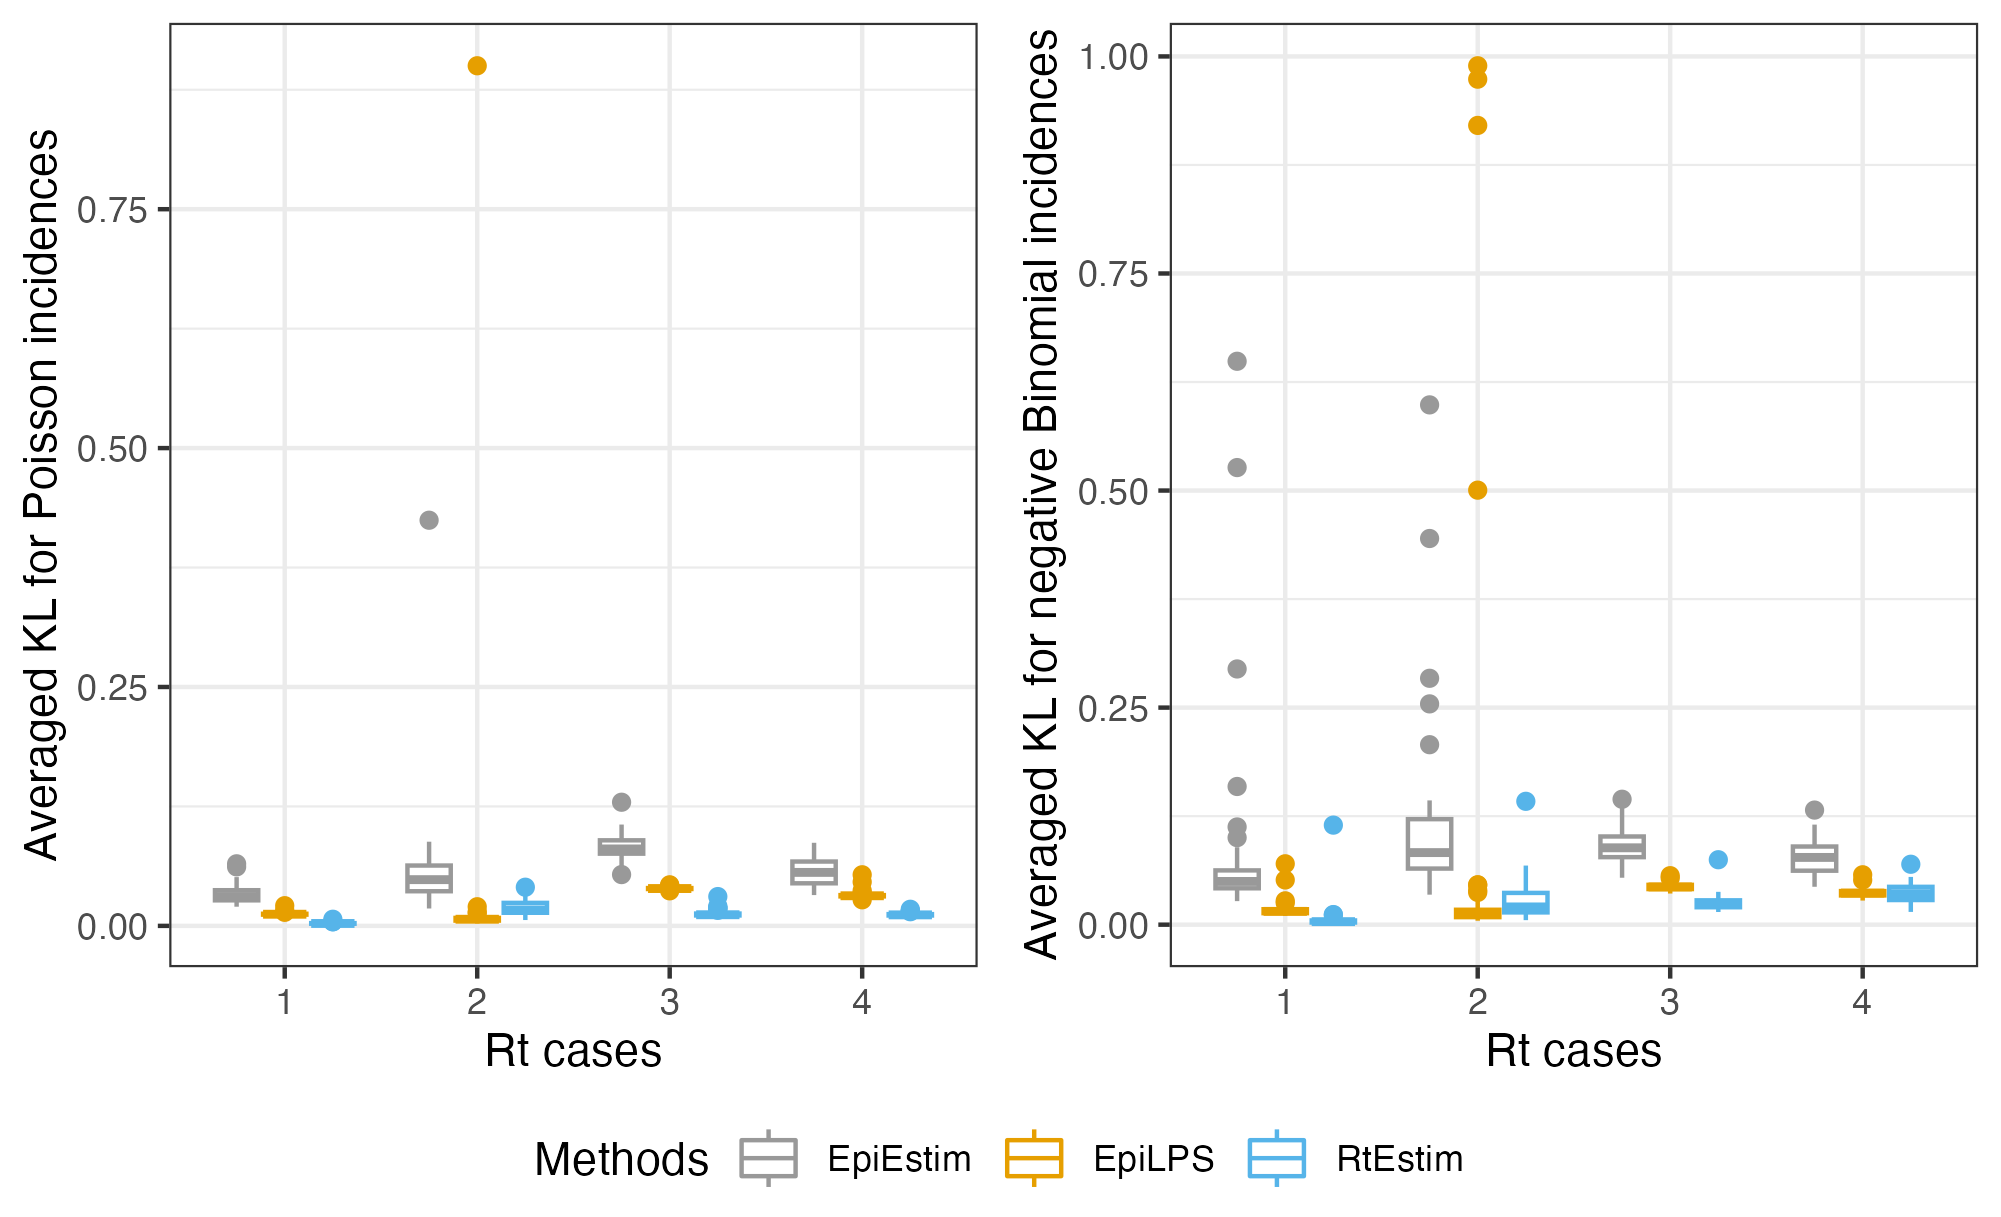
\includegraphics[width=.9\textwidth]{fig/kl.png}
    \caption{Boxplot of Kullback-Leibler divergence between the estimated effective reproduction numbers and the true ones across all methods given Poisson incidences and negative Binomial incidences across 50 samples. Left panel visualizes the KL divergences for the Poisson incidence cases. Right panel displays the KL divergences for the negative Binomial incidence cases.}% Outliers (larger than $3$) of EpiEstim is excluded for a better visualization.} 
    \label{fig:kl-res}
\end{figure}



% experiment results
\autoref{fig:pois-est} shows 1 realization for the estimated reproduction
numbers under the Poisson generative model for all 4 scenarios. Compared to
\EpiEstim\ and \EpiLPS, which have rather severe difficulties at the beginning
of the time series, \RtEstim\ estimates are more accurate---they nearly overlap
with the true values---without suffering from the edge problem. Scenario 2 is a
difficult problem for all methods: the sharp increase at the end of the stage of
exponential growth is difficult to capture. Although the truth is piecewise
exponential and likely best represented with a piecewise cubic curve, the actual
curvature is so gentle that linear estimation ($k=1$) appears potentially
reasonable. We, therefore, fit piecewise linear and cubic $\hat{\calR}_t$ curves
using \RtEstim\ for Scenario 2 to evaluate model misspecification. However, both
cases have difficulty recovering the acute rise in the growth phase. An
explanation of such failure is that the model imposes continuity at the
changepoint, which hinders the estimates from fitting the two discontinuous
phases. Scenario 1 is the simplest case with only one knot and two constant
segments. Besides the edge problem, \EpiEstim\ and \EpiLPS\ produce ``smooth''
estimated curves that are continuous at the changepoint, which results in
large mistakes in that neighbourhood. Since the
piecewise constant \RtEstim\ estimator does force any smoothness in
$\calR_t$, it easily captures the sharp decrease change. 

\begin{figure}[tb]
    \centering
    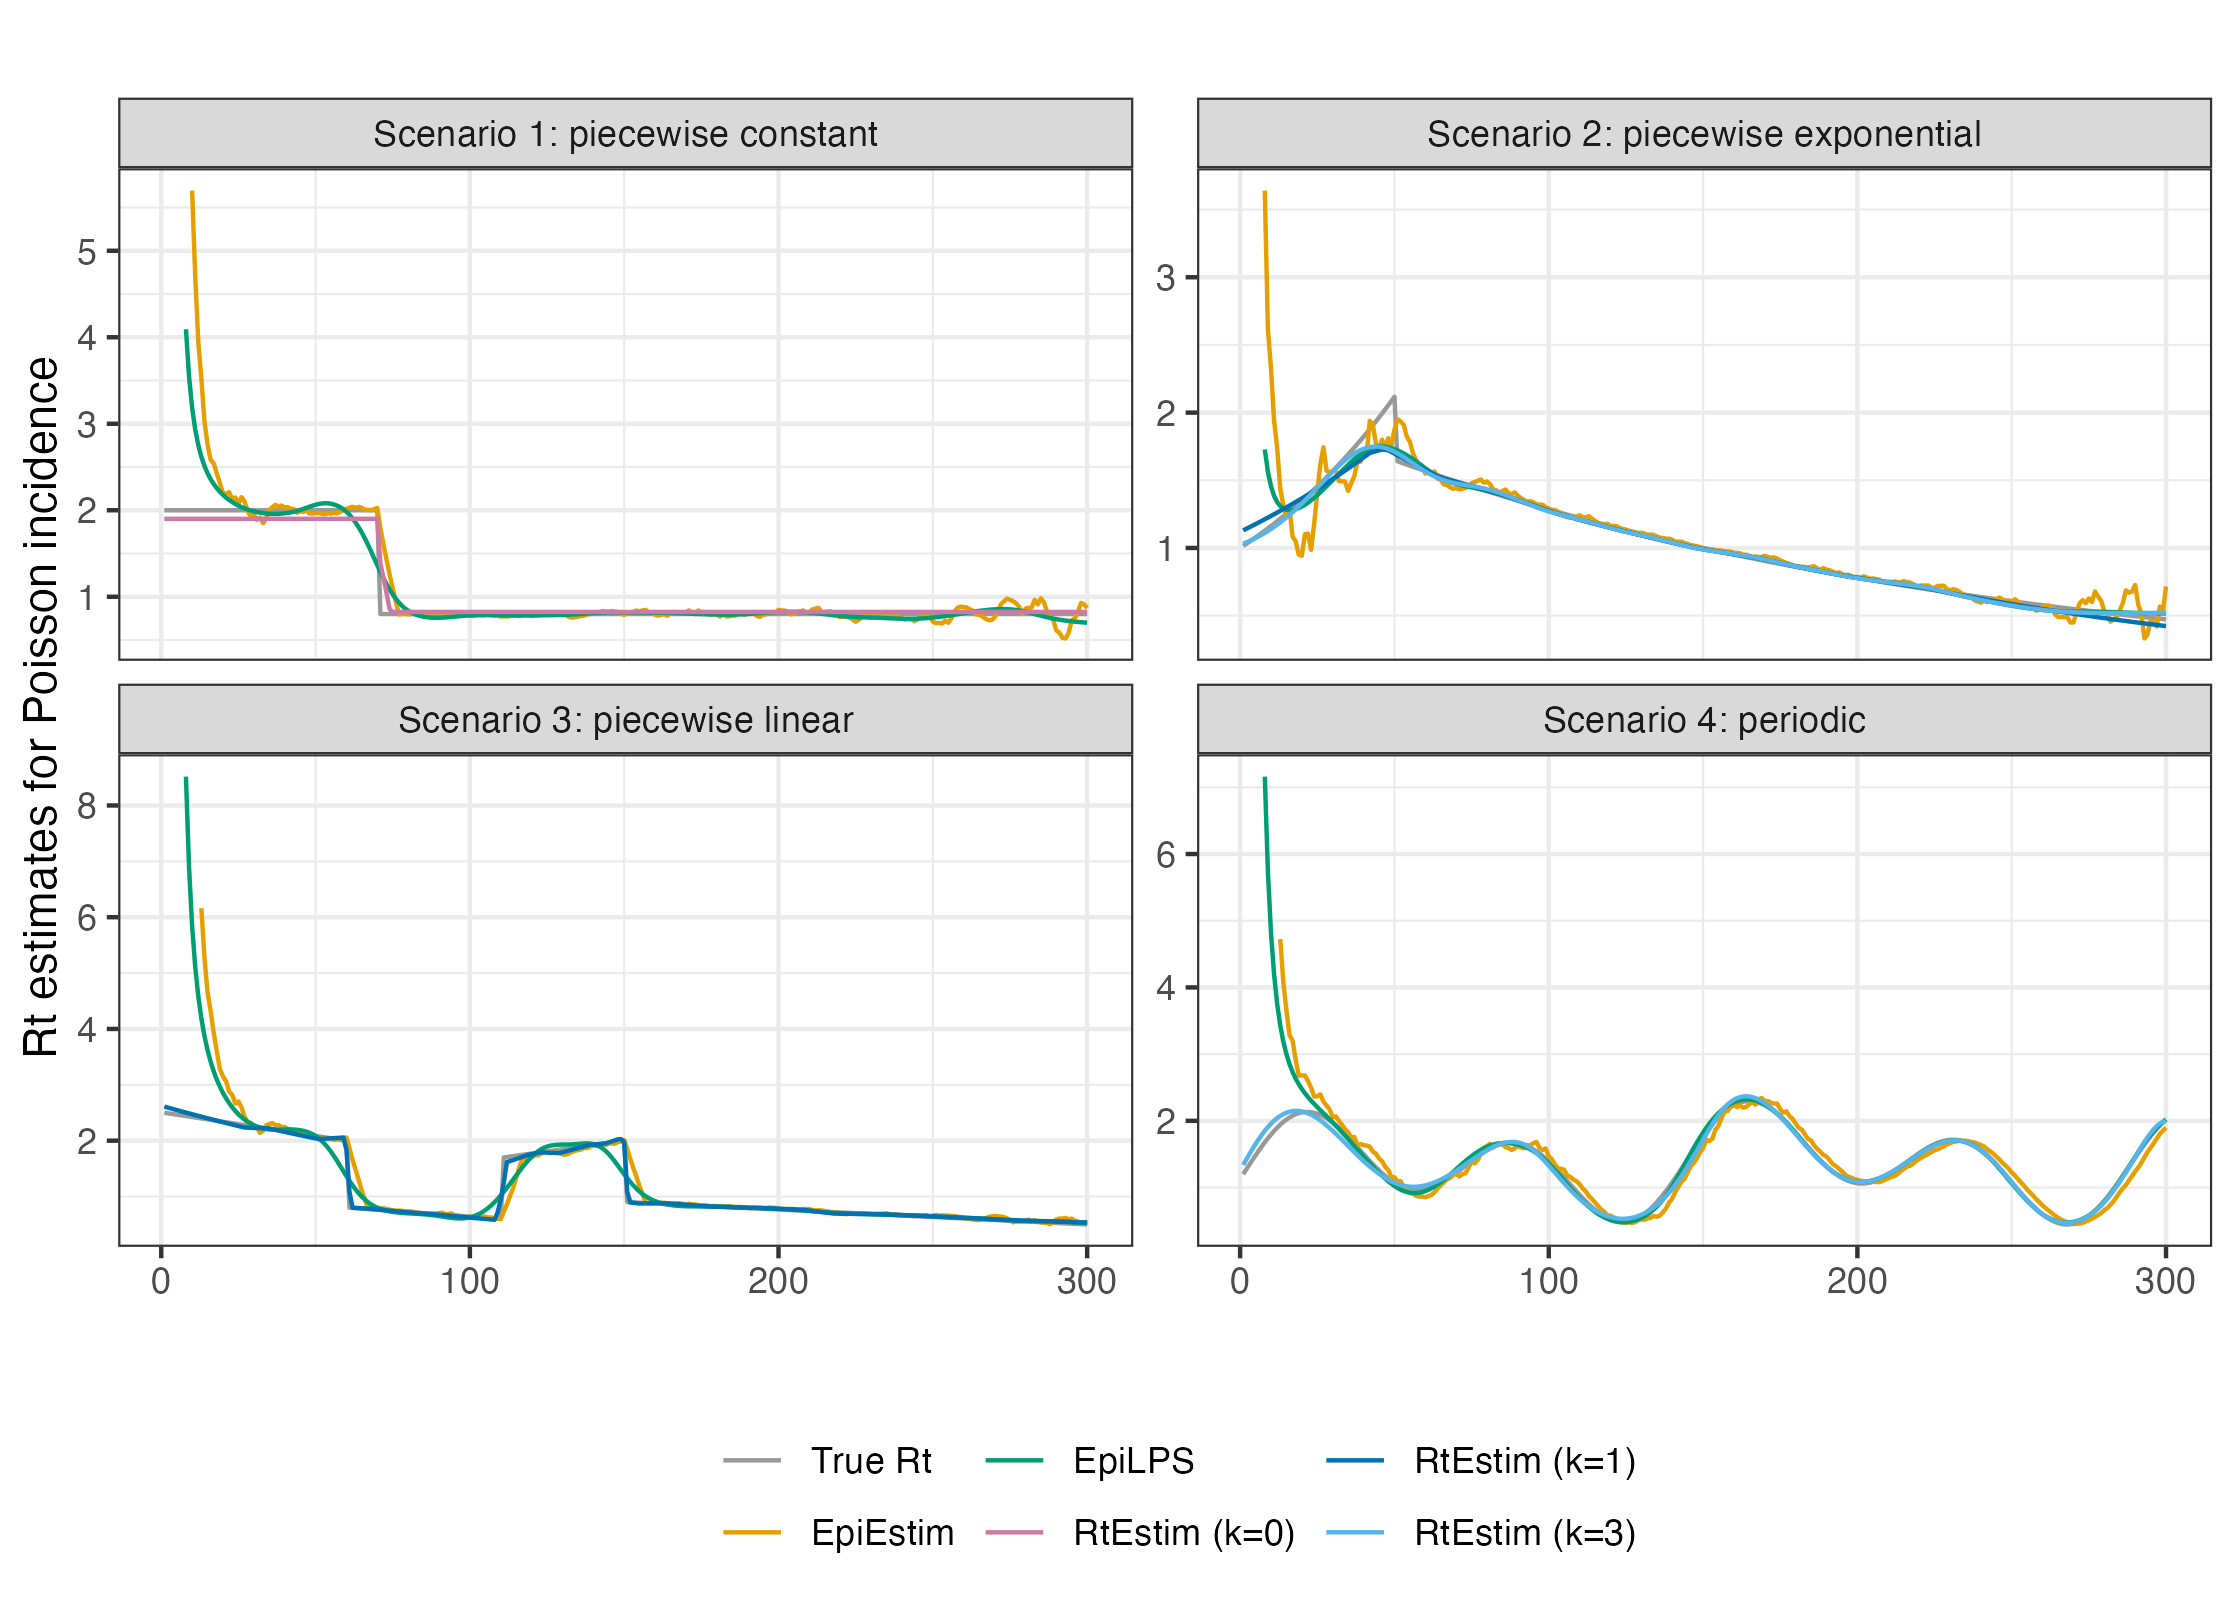
\includegraphics[width=.9\textwidth]{fig/Pois-res-plot.png}
    \caption{Effective reproduction number estimation for Poisson data.
    \texttt{RtEstim (k=1)} is the alternative estimation using $k=1$ in Scenario
    2. \attn{I'm not sure what this means. Can you fix the y-axis and (in the
    legend) put \texttt{RtEstim (k=?)} with a space for both cases.}}
    \label{fig:pois-est}
\end{figure}


% experiment results under the violation of assumptions
To investigate the performance under the violation of the Poisson distributional
assumption (of both \RtEstim\ and \EpiEstim), we also examine estimation
accuracy with negative Binomial data. \autoref{fig:nb-est} displays a
realization, analogous to the previous case, for all methods and scenarios.
\RtEstim\ has more difficulty relative to the Poisson incidence cases,
especially at the beginning of the outbreak. This is most pronounced in Scenario
4, where \RtEstim\ is overly smooth, except in the last wave. In Scenario 2,
\RtEstim\ successfully captures the changepoint, but suffers from the same
problem as in the Poisson setting. In Scenario 3, the piecewise linear \RtEstim\
recovers the curvature of $\calR_t$ well, but is less accurate than
in the Poisson incidence cases.

\begin{figure}[tb]
    \centering
    \includegraphics*[width=.9\textwidth]{fig/NB-res-plot.png}
    \caption{Effective reproduction number estimation for negative Binomial
    incidences. \texttt{RtEstim (k=1)} is the alternative estimation using $k=1$
    in Scenario 2. \attn{see comments on previous figure.}}
    \label{fig:nb-est}
\end{figure}

Finally, it is important to provide a brief comparison of the running times of
three models across the $8$ experimental settings. We find that almost all
models across all experiments complete within $10$ seconds to converge.
\RtEstim\ generally takes the longest, likely due to a relatively large
candidate set---$50$ values of $\lambda$ and 3 folds of cross validation---while
other models only run a single time for a fixed setting of hyperparameters per
experiment. Additional results on timing comparisons are deferred to the
supplementary document. 



\subsection{Real-data results: Covid-19 incident cases in British Columbia}

% introduce data & tuning parameter setup
We implement our \RtEstim\ on the Covid-19 confirmed cases in British Columbia
(B.C.) as of May 18, 2023 (visualized in \autoref{fig:covid-data}) reported by
B.C. Centre for Disease Control. The reported incidence cases provide a snapshot
of how testing recommendations and practices have changed over the three years.
We choose the gamma distribution with shape $2.5$ and scale $2.5$ to approximate
the serial interval function, which is empirically found to be a reasonable
choice. 

\begin{figure}[tb]
    \centering
    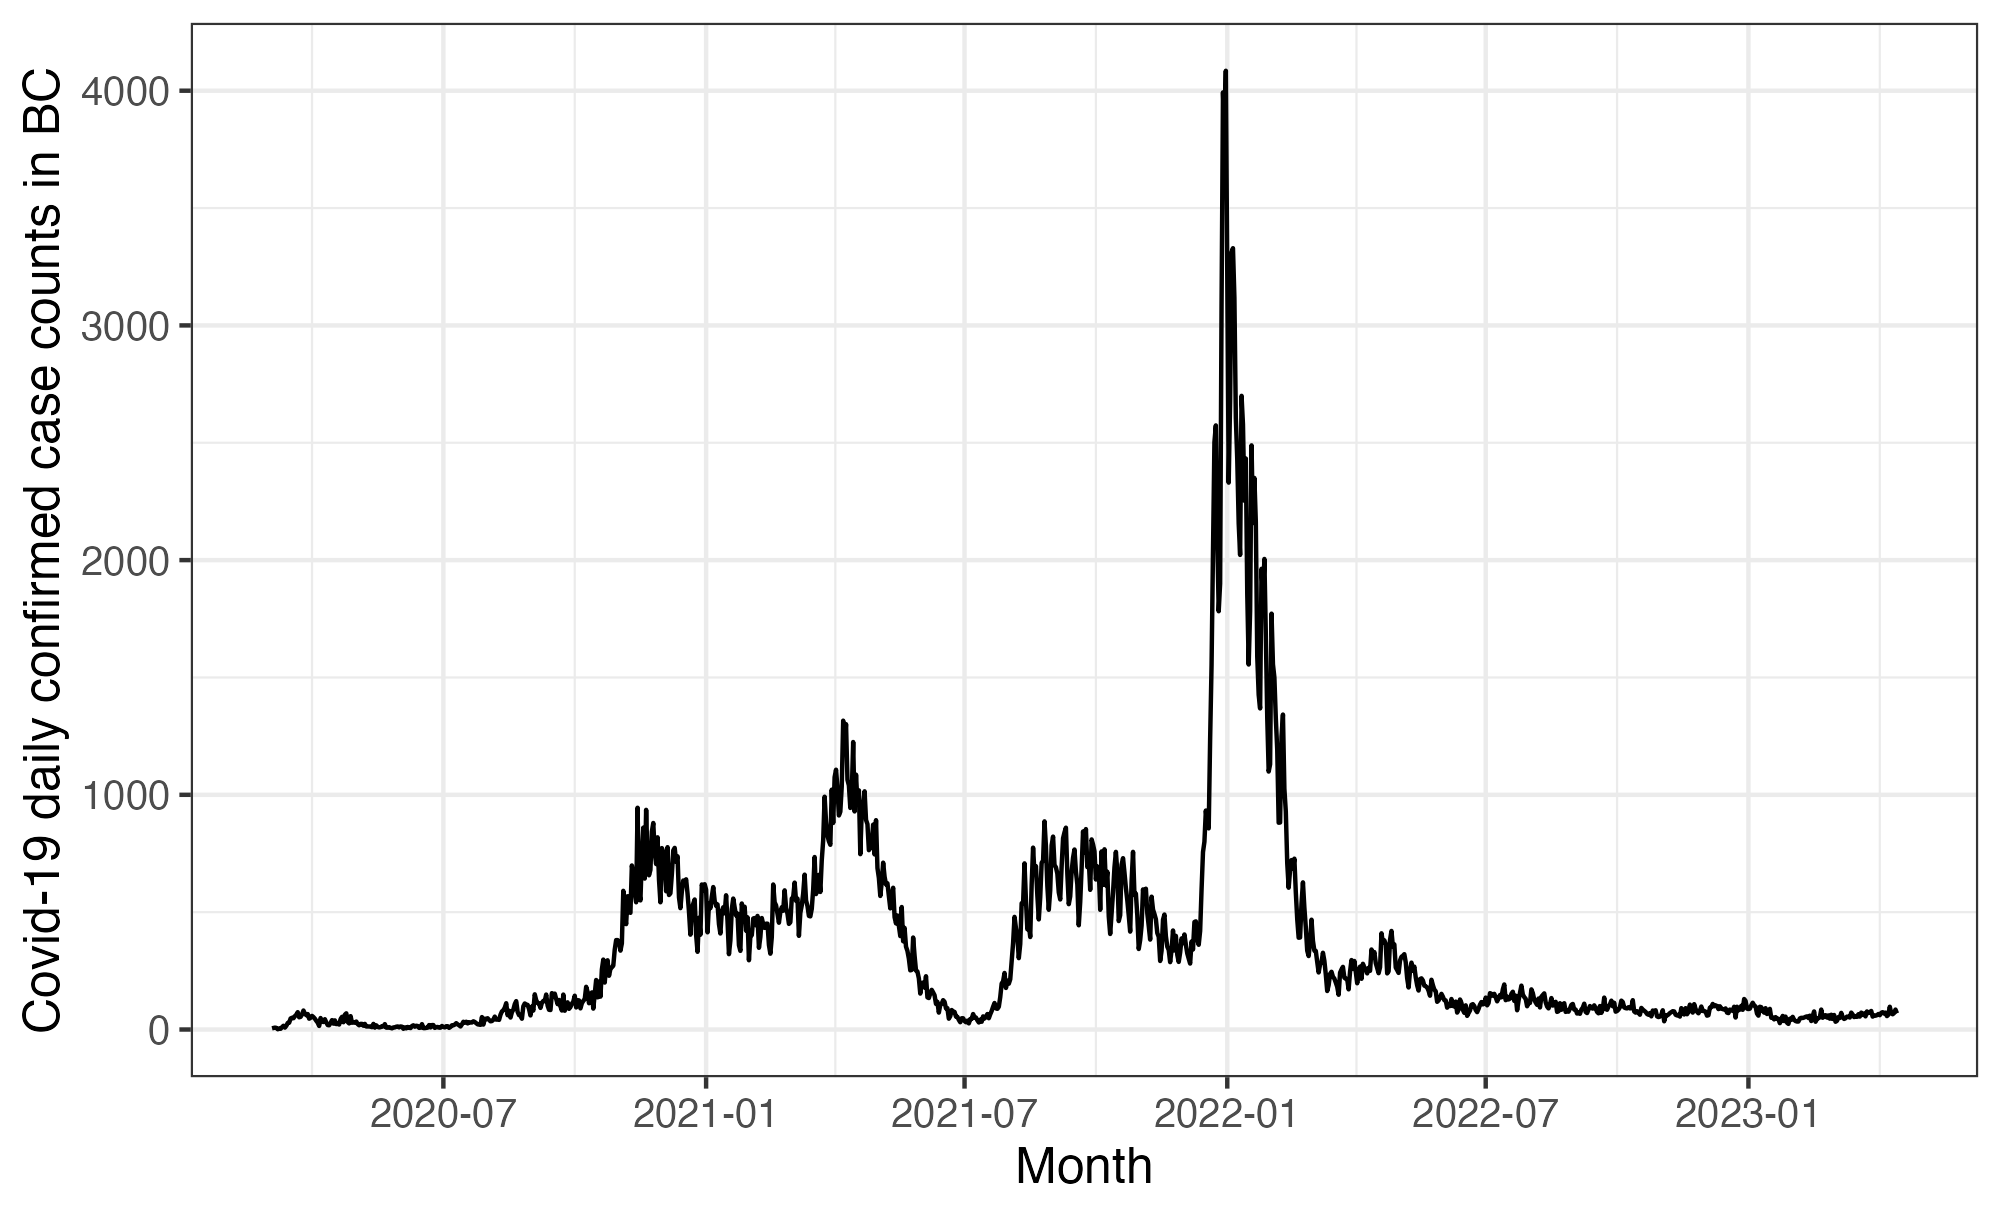
\includegraphics[width=0.9\textwidth]{fig/covid_dat.png}
    \caption{Covid19 daily confirmed incidence counts between March 1st, 2020 and April 15th, 2023 in British Columbia, Canada.} 
    \label{fig:covid-data}
\end{figure} 

% interpret figures -- across all lambdas
Considering the temporal evolutions of effective reproduction numbers across $3, 4, 5$ days, the estimated reproduction numbers of Covid-19 in British Columbia (illustrated in \autoref{fig:covid-rt}) are less than $3$ during most of the time, which means that one distinct infected individuals can on average infect less than three other individuals in the population. The three degrees of the temporal evolution (across all regularization levels $\lambda$) all yield similar results that $\hat{\calR}_t$ comes to the highest peak around the end of 2021 and then drops down to the lowest trough shortly thereafter. Throughout the estimated curves, the peaks and troughs of the reproduction numbers roughly come prior to the following growths and decays of confirmed cases respectively.
% CBs for real epidemic applications
We also visualize the 95\% empirical confidence bands of the point estimates for the ``best'' tuning parameter (in terms of MSEs). 

The reproduction numbers are relatively unstable before April 1st, 2022. The highest peak coincides with the emergence and globally spread of the Omicron variant. The estimated reproduction numbers are apparently below the threshold $1$ during two time periods -- roughly from April 1st, 2021 to July 1st, 2021 and from January 1st, 2022 to April 1st, 2022. The first trough coincides with the first authorization for use of Covid-19 vaccines in British Columbia. The second trough shortly after the greatest peak may credit to many aspects, including self-isolation of the infected individuals and application of the second shot of Covid-19 vaccines. Since around April 1st, 2022, the reproduction numbers stay stable (fluctuating around $1$) and the infected cases stay low. 

% for different lambda
Greater regularization levels (by using larger $\lambda$s) result in smoother
estimated curves. Smoother curves suggest that the estimated reproduction
numbers are around $1$ during most time periods; however, it may miss to capture
some outbreaks of the pandemic. More wiggly curves better reflect the
fluctuation of $\calR_t$, but sometimes fail to highlight the significant peaks
or troughs. The tuning parameter $\lambda$ needs to be chosen corresponding to
the information in practice for a better interpretation. Here, we provide the
CV-chosen $\calR_t$ estimates with confidence bands. 

\begin{figure}[tb]
    \centering
    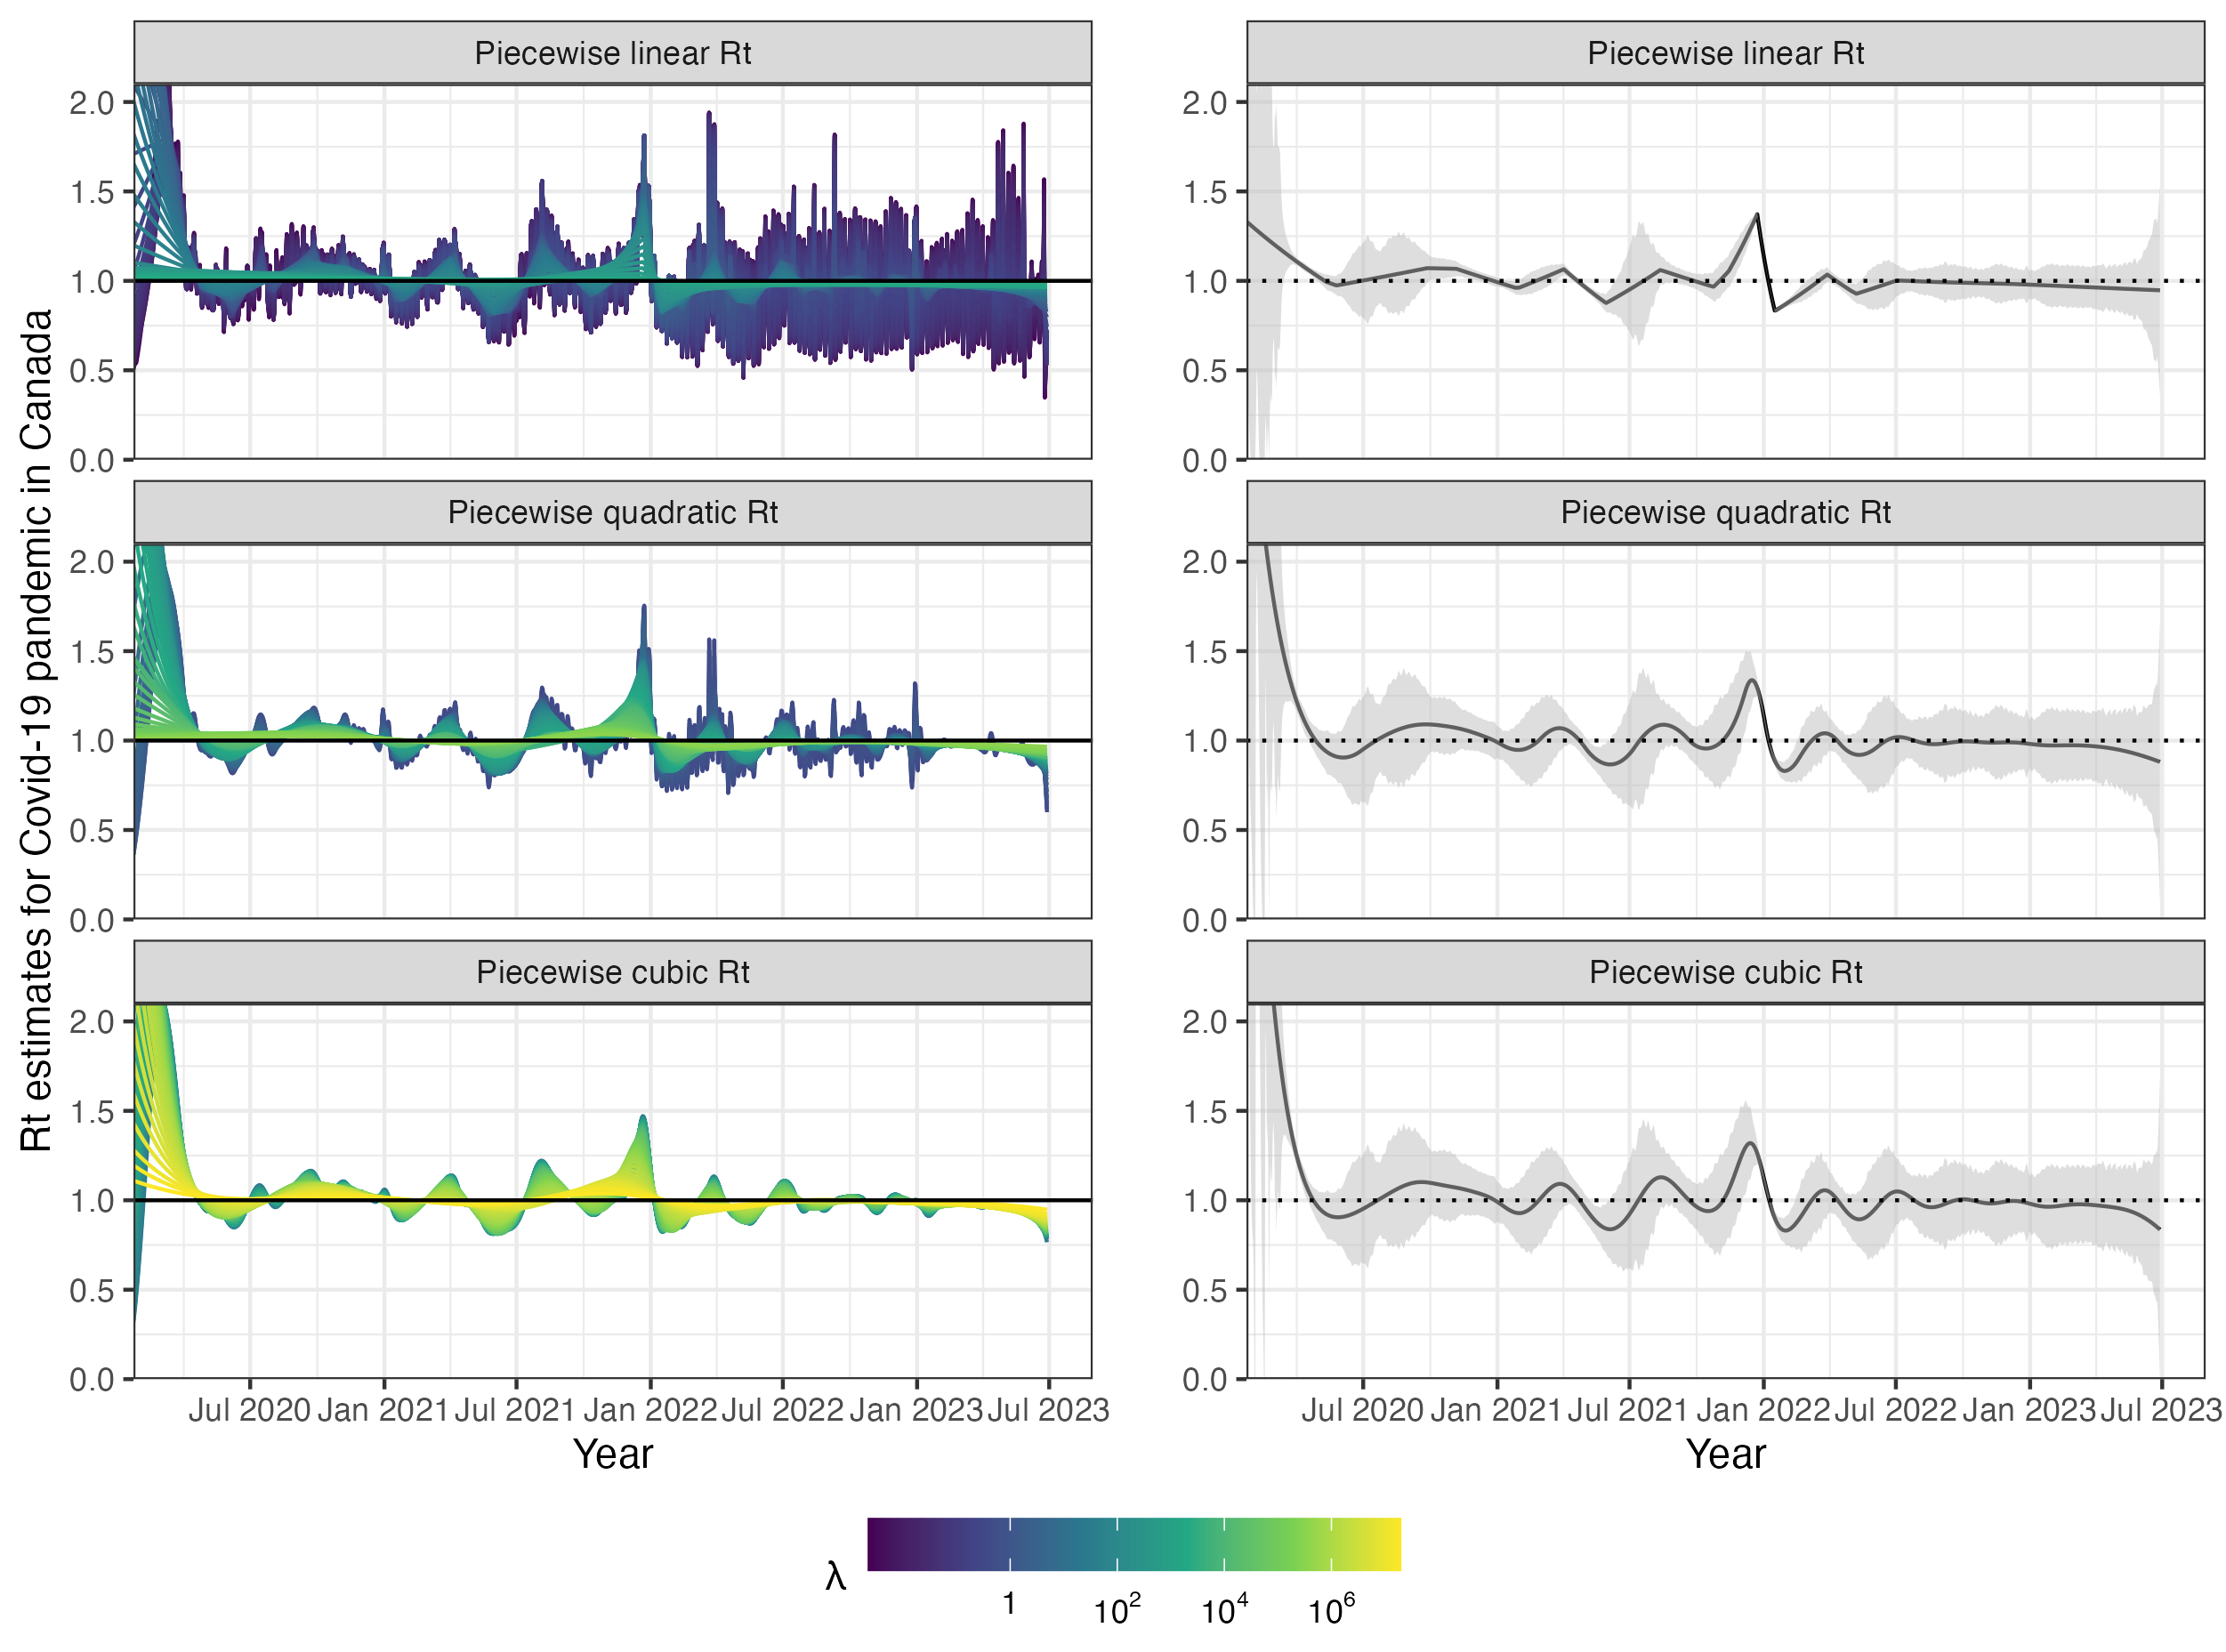
\includegraphics[width=0.9\linewidth]{fig/covid_full_res.png}
    \caption{Estimated effective reproduction numbers for Covid19 daily confirmed counts between March 1st, 2020 and April 15th, 2023 in British Columbia, Canada. The left panels display the CV-tuned estimates with 95\% confidence intervals. The right panels demonstrate estimates corresponding to 50 tuning parameters. The top, medium and bottom panels illustrate the estimated reproduction numbers ($\calR_t$) using the Poisson trend filtering (in \eqref{eq:rt-ptf}) with degrees $k=1,2,3$ respectively.} 
    \label{fig:covid-rt}
\end{figure} 


\subsection{Pandemic influenza in Baltimore, Maryland, 1918}

We then apply \RtEstim\ on the pandemic influenza in Baltimore, Maryland, 1918. Dataset in \autoref{fig:flu-dat} is obtained from the \texttt{R} package \EpiEstim. The 1918 influenza, caused by H1N1 influenza A virus, was an unprecedentedly deadly influenza that infected almost one-third of the population across the world \citep{taubenberger20061918}. 
In the estimation displayed in \autoref{fig:flu-res}, the CV-tuned piecewise
cubic estimates better capture the growing tendency at the beginning of the
pandemic. It suggests that the pandemic has yielded a decrease after around 20
days and reached $1$ when the pandemic has lasted for nearly 50 days. However,
it also suggests an increase at the end of the period, while a steady decline
(as in CV-tuned piecewise constant and linear estimates) is more reasonable. The
smoothness of $\calR_t$ curves should be chosen based on the purpose of the
study in practice, e.g., epidemic forecasting may require a more wiggly curve
that contains more fluctuation information, while retrospective studies that
solely target on understanding of the pandemic may prefer a smoother curve with
less important information smoothed out. 

\begin{figure}[tb]
    \centering
    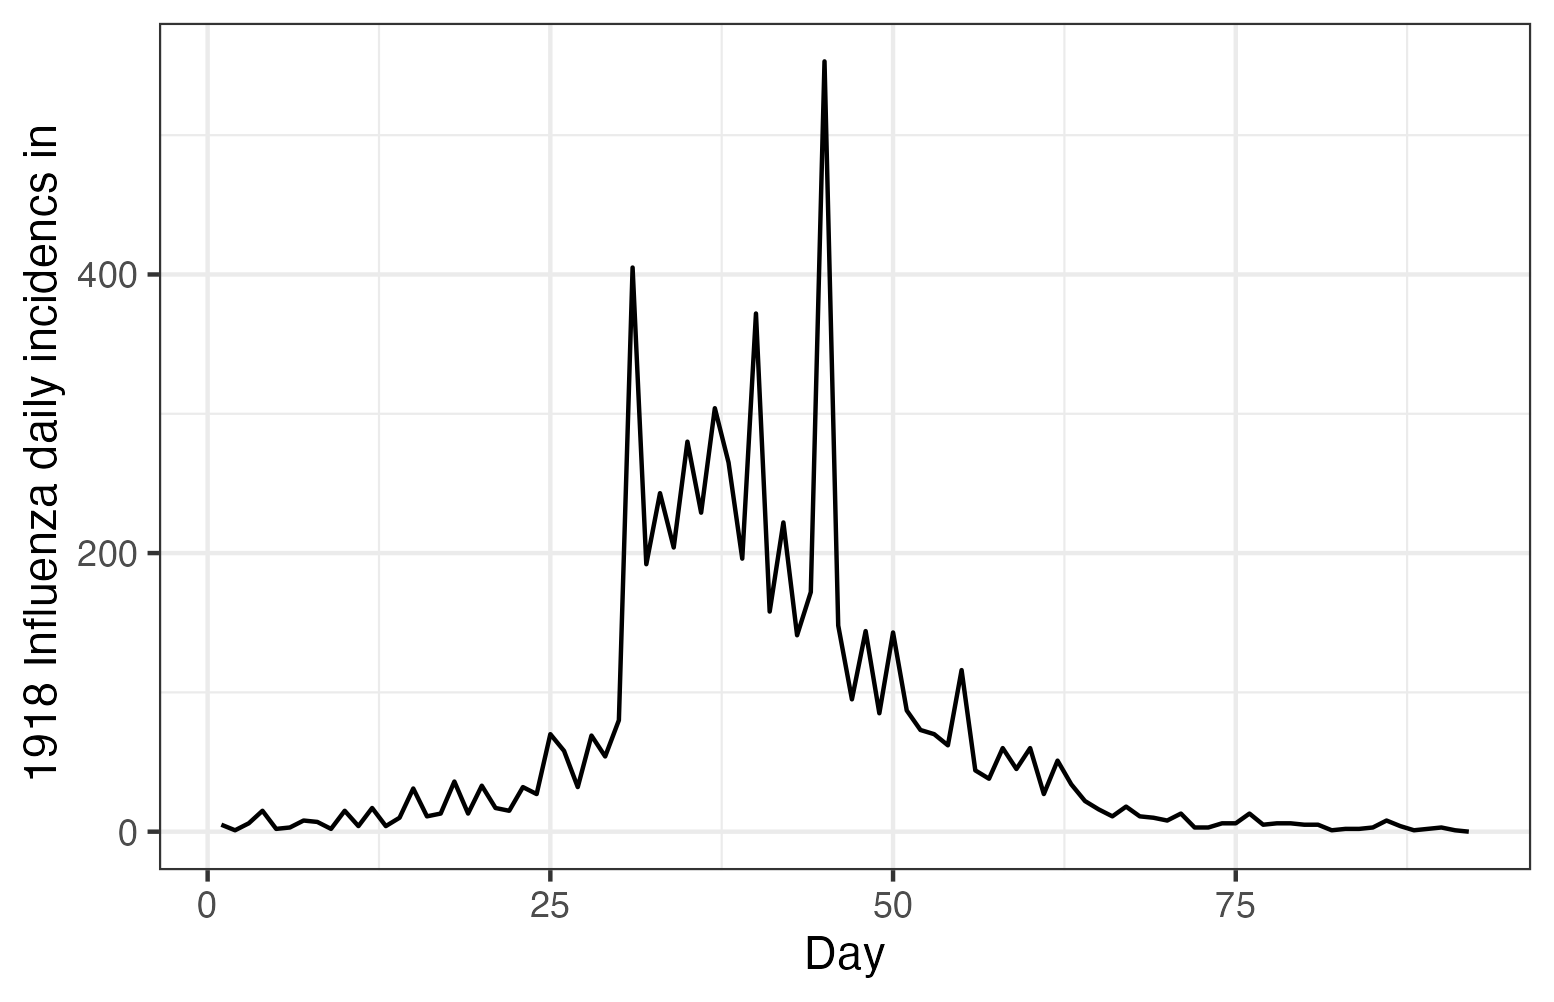
\includegraphics[width=0.9\linewidth]{fig/flu_dat.png}
    \caption{Pandemic influenza incidence counts in Baltimore, Maryland in 1918.} 
    \label{fig:flu-dat}
\end{figure} 

\begin{figure}[tb]
    \centering
    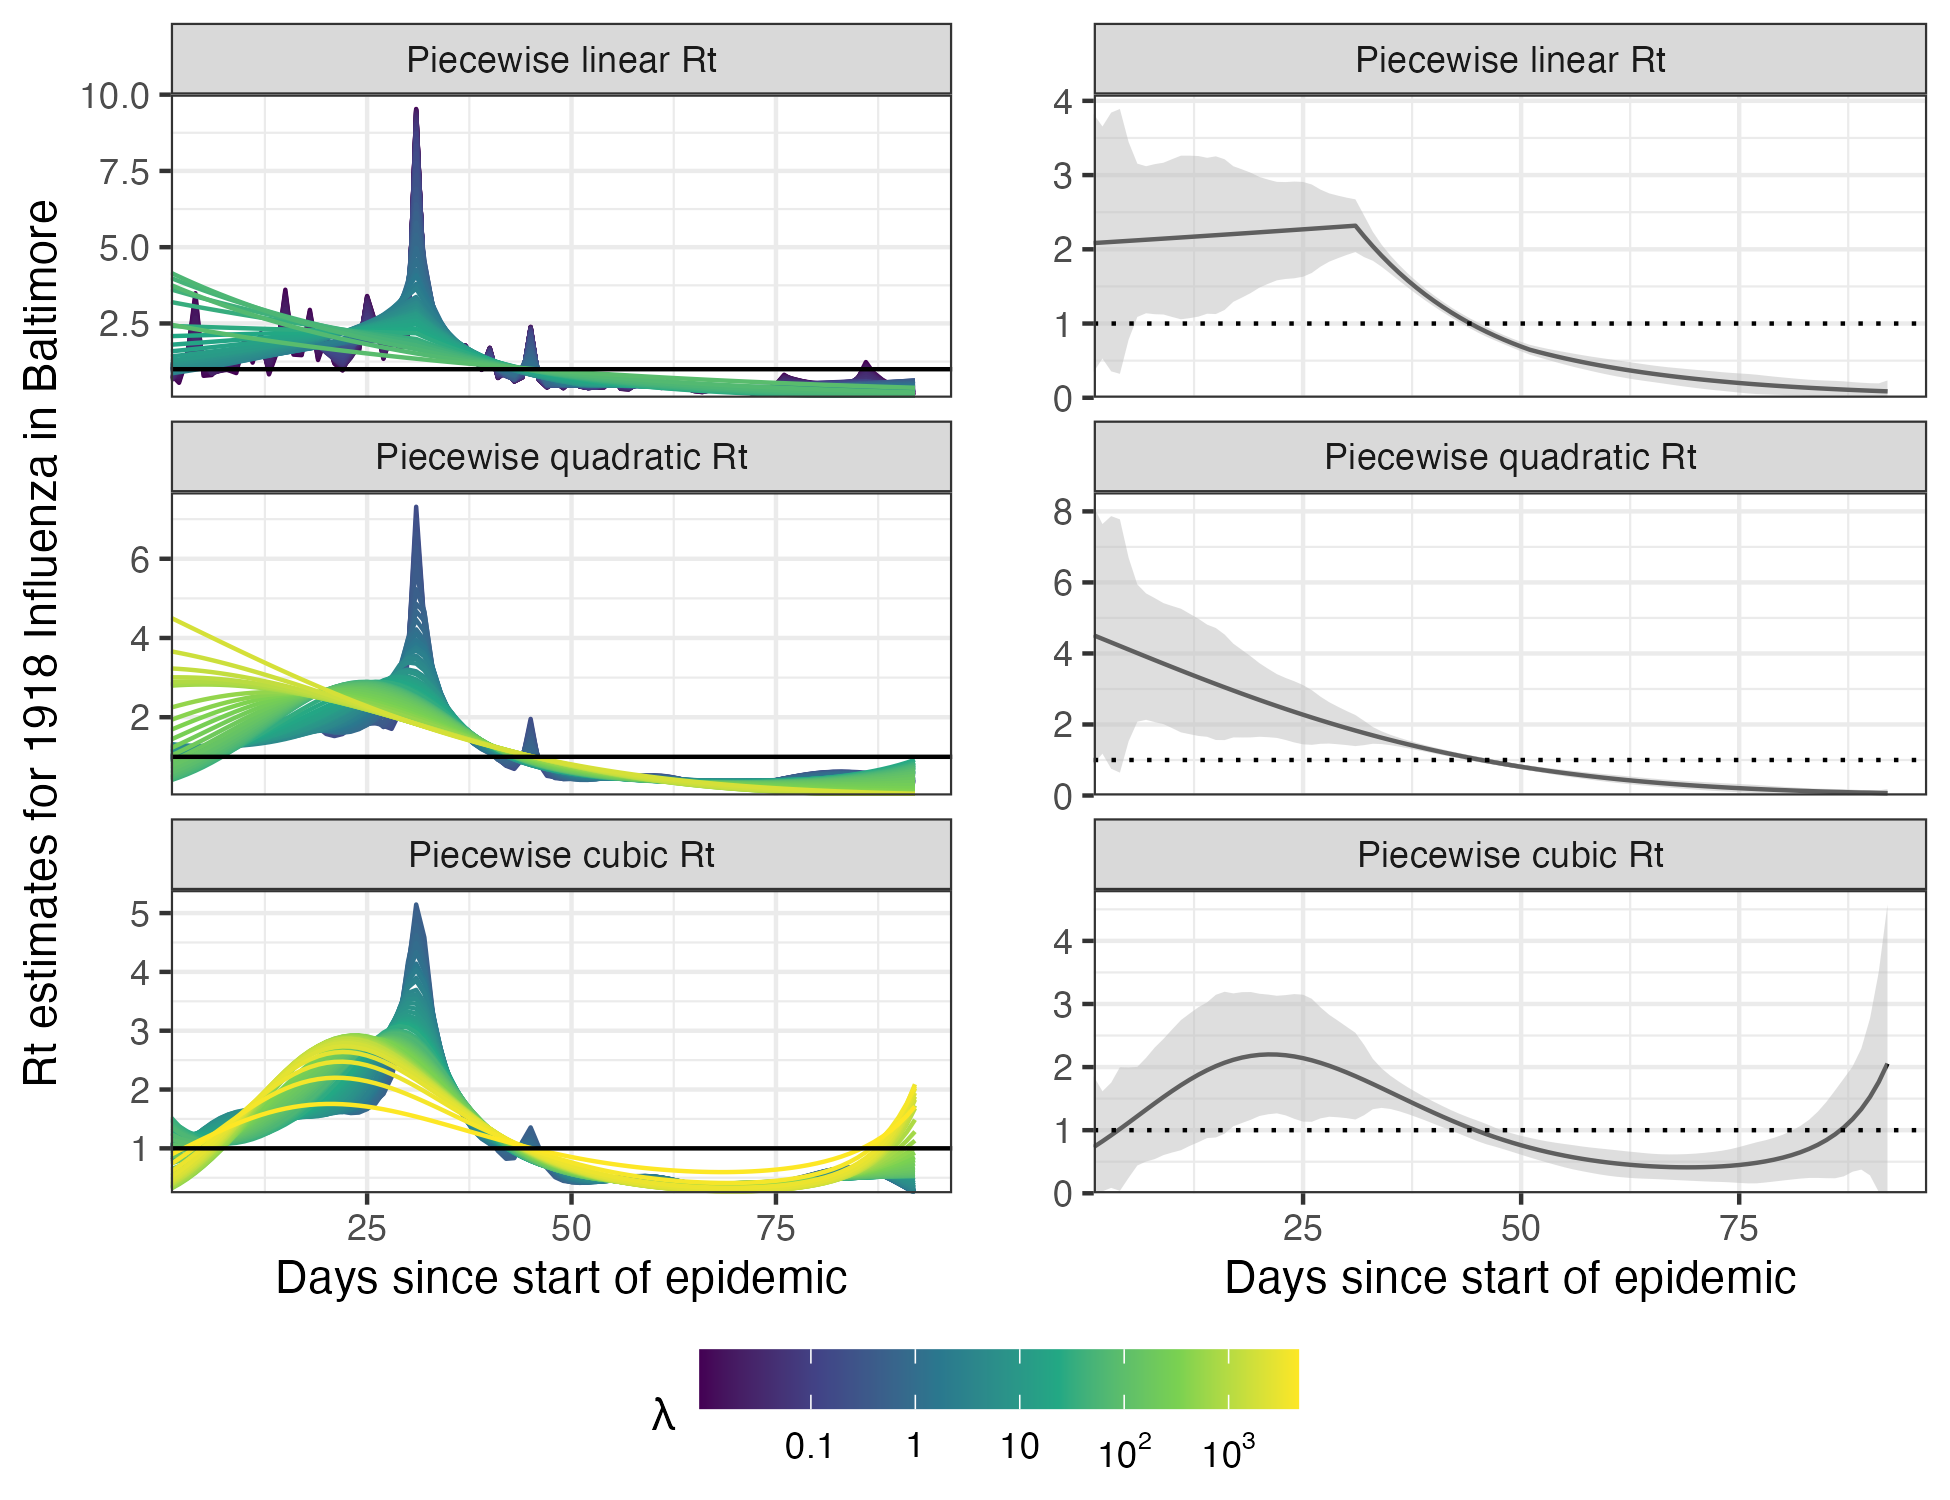
\includegraphics[width=0.9\linewidth]{fig/flu_full_res.png}
    \caption{Estimated effective reproduction numbers for pandemic influenza incidence counts in Baltimore, Maryland in 1918. The left panels display the CV-tuned estimates with 95\% confidence intervals. The right panels demonstrate estimates corresponding to 50 tuning parameters. The top, medium and bottom panels illustrate the estimated reproduction numbers ($\calR_t$) using the Poisson trend filtering (in \eqref{eq:rt-ptf}) with degrees $k=1,2,3$ respectively.} 
    \label{fig:flu-res}
\end{figure} 

